\section{The Rosenbrock Function}
\label{sec:rosenbrock_function}

  Introduced by Howard H. Rosenbrock in 1960\footnote{
    Rosenbrock, H.H. (1960). \enquote{An automatic method for finding the
    greatest or least value of a function}. The Computer Journal. 3 (3): 
    175-184. doi:10.1093/comjnl/3.3.175. ISSN 0010-4620.
  }, the Rosenbrock function is a non-convex function that serves as a benchmark
  for optimization algorithms.
  Despite its simplicity, it poses a challenge due to its characteristic
  landscape, a long, narrow, parabolic-shaped flat valley.
  While finding the valley is relatively simple, converging to the global
  minimum within it is notably difficult.

  \begin{definition}[Rosenbrock function]
    \label{def:rosenbrock_function}
    The \emph{Rosenbrock function}, denoted as \(f: \mathbb{R}^n \rightarrow 
    \mathbb{R}\), is defined by the following equation:

    \begin{equation}
    \label{eq:rosenbrock_function}
      f(\mathbf{x}) 
        = \sum_{i=1}^{n-1} \left[ 
          100 (\mathbf{x}_{i+1} - \mathbf{x}_i^2)^2 + (1 - \mathbf{x}_i)^2 
        \right]
    \end{equation}

    In this equation:

    \begin{itemize}
      \item \(n\) is the number of dimensions.
      \item \(\mathbf{x}\) is a vector composed of \(n\) real numbers.
    \end{itemize}
  \end{definition}

  The Rosenbrock function's global minimum is at \(f(\mathbf{x}^*) = 0\), 
  corresponding to the point \(\mathbf{x}^* = (1, \ldots, 1)\).
  To illustrate the function's behavior for \(n = 2\), 
  \vref{fig:rosenbrock_function} presents a contour plot and a surface plot.

  \begin{figure}[ht!]
    \centering
    \begin{subfigure}[b]{0.4\textwidth}
      \centering
      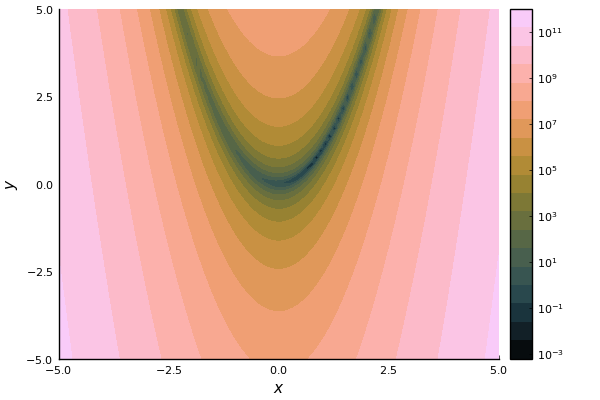
\includegraphics[width=\textwidth]{img/test_functions/rosenbrock_contour.png}
    \end{subfigure}
    \begin{subfigure}[b]{0.4\textwidth}
      \centering
      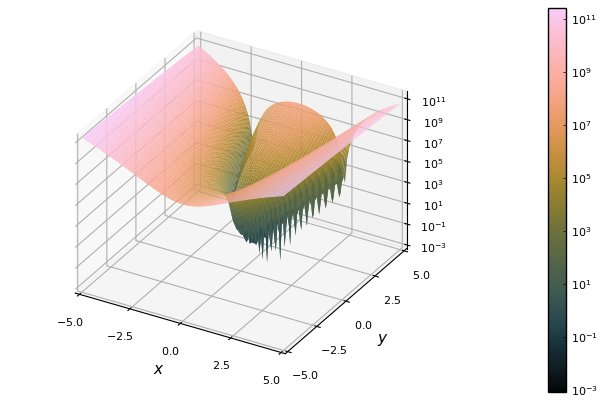
\includegraphics[width=\textwidth]{img/test_functions/rosenbrock_surface.png}
    \end{subfigure}
    \caption{Rosenbrock Function for \(n = 2\)}
    \label{fig:rosenbrock_function}
  \end{figure}
